%%%%%%%%%%%%%%%%%%%%%%%%%%%%%%%%%%%%%%%%%%%%%%%%%%%%%%%%%%%%%%%%%%%%%%%%%%%%%%%%%%%
%% Curtin Presentation Beamer Template                                           %%
%% Adapted from UFC template by
%% author: Maurício Moreira Neto - Doctoral student in Computer Science (MDCC)   %%
%%%%%%%%%%%%%%%%%%%%%%%%%%%%%%%%%%%%%%%%%%%%%%%%%%%%%%%%%%%%%%%%%%%%%%%%%%%%%%%%%%%

\documentclass{lib/curtin_format}
\usepackage{subcaption}
% Inserting the preamble file with the packages
%%%%%%%%%%%%%%%%%%%%%%%%%%%%%%%%%%%%%%%%%%%%%%%%%%%%%%%%%%%%%%%%%%%%%
%% This file contains the packages that can be used in the beamer. %%
%%%%%%%%%%%%%%%%%%%%%%%%%%%%%%%%%%%%%%%%%%%%%%%%%%%%%%%%%%%%%%%%%%%%%
% Package to fonts family
\usepackage[T1]{fontenc}
% Package to accentuation
\usepackage[utf8]{inputenc}
% Package to Portuguese language
%\usepackage[brazil]{babel}

%just in case eps figures are available instead - automatically converted to PDF
\usepackage{epstopdf}

% Package to Figures
\usepackage{graphicx}
% Package to the colors
\usepackage{color}
% Package to the colors
\usepackage{xcolor}
% Packages to math symbols and expressions
\usepackage{amsfonts, amssymb, amsmath}
% Package to multiple lines and columns in table
\usepackage{multirow, array} 
% Package to create pseudo-code
% For more detail of this package: http://linorg.usp.br/CTAN/macros/latex/contrib/algorithm2e/doc/algorithm2e.pdf
\usepackage{algorithm2e}
% Package to insert code
\usepackage{listings} 
\usepackage{keyval}
% Package to justify text
\usepackage[document]{ragged2e}
% Package to manage the bibliography
% \usepackage[backend=biber, style=numeric, sorting=none]{biblatex}
% Package to facilities quotations
\usepackage{csquotes}
% Package to use multicols
\usepackage{multicol}


% Inserting the references file
% \bibliography{references-crackseg.bib}
%\usepackage[style=author,backend=bibtex]{biblatex}
%\addbibresource{references.bib}

% \begin{figure}
%         \centering        
%         \includegraphics[width=2.00cm,height=1.00cm]{figs/ICONIP2021_logo.eps}
%         %\caption{Example of semantic segmentation}        
%         \label{fig:logo}
% 	\end{figure}	
% \vspace{-0.4cm}

% Title
\title[SC-CrackSeg]{\huge\textbf{SC-CrackSeg: A Real-time Shared Feature Pyramid
Network for Crack Detection and Segmentation}}
% Subtitle
%\subtitle{ICONIP 2021}

% Author of the presentation
\author{Moritz Bergemann \\ Supervised by Aneesh Krishna and Sonny Pham}
% Institute's Name
\institute[Curtin]{
    % email for contact
    \normalsize{\email{}}
    \newline
    % Department Name
    \department{School of EECMS}
    %\newline
    % university name
    \curtin
}
% date of the presentation
\date{}


%%%%%%%%%%%%%%%%%%%%%%%%%%%%%%%%%%%%%%%%%%%%%%%%%%%%%%%%%%%%%%%%%%%%%%%%%%%%%%%%%%
%% Start Document of the Presentation                                           %%               
%%%%%%%%%%%%%%%%%%%%%%%%%%%%%%%%%%%%%%%%%%%%%%%%%%%%%%%%%%%%%%%%%%%%%%%%%%%%%%%%%%
\begin{document}
% insert the code style
%%%%%%%%%%%%%%%%%%%%%%%%%%%%%%%%%%%%%%%%%%%%%%%%%%%%%%%%%%%%%%%%%%%%%%%%%%%%%%%%%%%
%% This file contains the style of the codes show in slides.                     %%
%% The package used is listings, but it possible to used others.                 %%
%%%%%%%%%%%%%%%%%%%%%%%%%%%%%%%%%%%%%%%%%%%%%%%%%%%%%%%%%%%%%%%%%%%%%%%%%%%%%%%%%%%

% color used in the code style
\definecolor{codegreen}{rgb}{0,0.6,0}
\definecolor{codegray}{rgb}{0.5,0.5,0.5}
\definecolor{codepurple}{rgb}{0.58,0,0.82}
\definecolor{codebackground}{rgb}{0.95,0.95,0.92}

% style of the code!
\lstdefinestyle{codestyle}{
    backgroundcolor=\color{codebackground},   
    commentstyle=\color{codegreen},
    keywordstyle=\color{magenta},
    numberstyle=\tiny\color{codegray},
    stringstyle=\color{codepurple},
    basicstyle=\ttfamily\footnotesize,
    frame=single,
    breakatwhitespace=false,         
    breaklines=true,                 
    captionpos=b,                    
    keepspaces=true,                 
    numbers=left,                    
    numbersep=5pt,                  
    showspaces=false,                
    showstringspaces=false,
    showtabs=false,                  
    tabsize=2,
    title=\lstname 
}

\lstset{style=codestyle}


%% ---------------------------------------------------------------------------
% First frame (with tile, subtitle, ...)
\begin{frame}{}	

    \maketitle
	\vspace{-0.4cm}
	\begin{figure}
        \centering        
        %\caption{Example of semantic segmentation}        
        \label{fig:logo}
	\end{figure}	

\end{frame}

%% ---------------------------------------------------------------------------
% Second frame
\begin{frame}{Table of Contents}
    %\begin{multicols}{2}
        \tableofcontents
    %\end{multicols}
\end{frame}

%% ---------------------------------------------------------------------------
% This presentation is separated by sections and subsections
\section{Overview of key contributions}
\begin{frame}{Overview of key contributions}
Our key contributions are:
	\begin{itemize}
		\item Introduce a new state-of-the-art model specifically designed for crack segmentation application task
		\item Assessed the unexplored field of domain adversarial semantic segmentation using transfomer models
		\item Evaluated lightweight segmentation transformers for unsupervised domain adaptation, and introduced novel pseudo-teacher approach for state-of-the-art results
	\end{itemize}
\end{frame}


\section{Crack Segmentation}
\begin{frame}{Crack Segmentation}
\vspace{0.1cm}
\begin{figure}
    \centering
    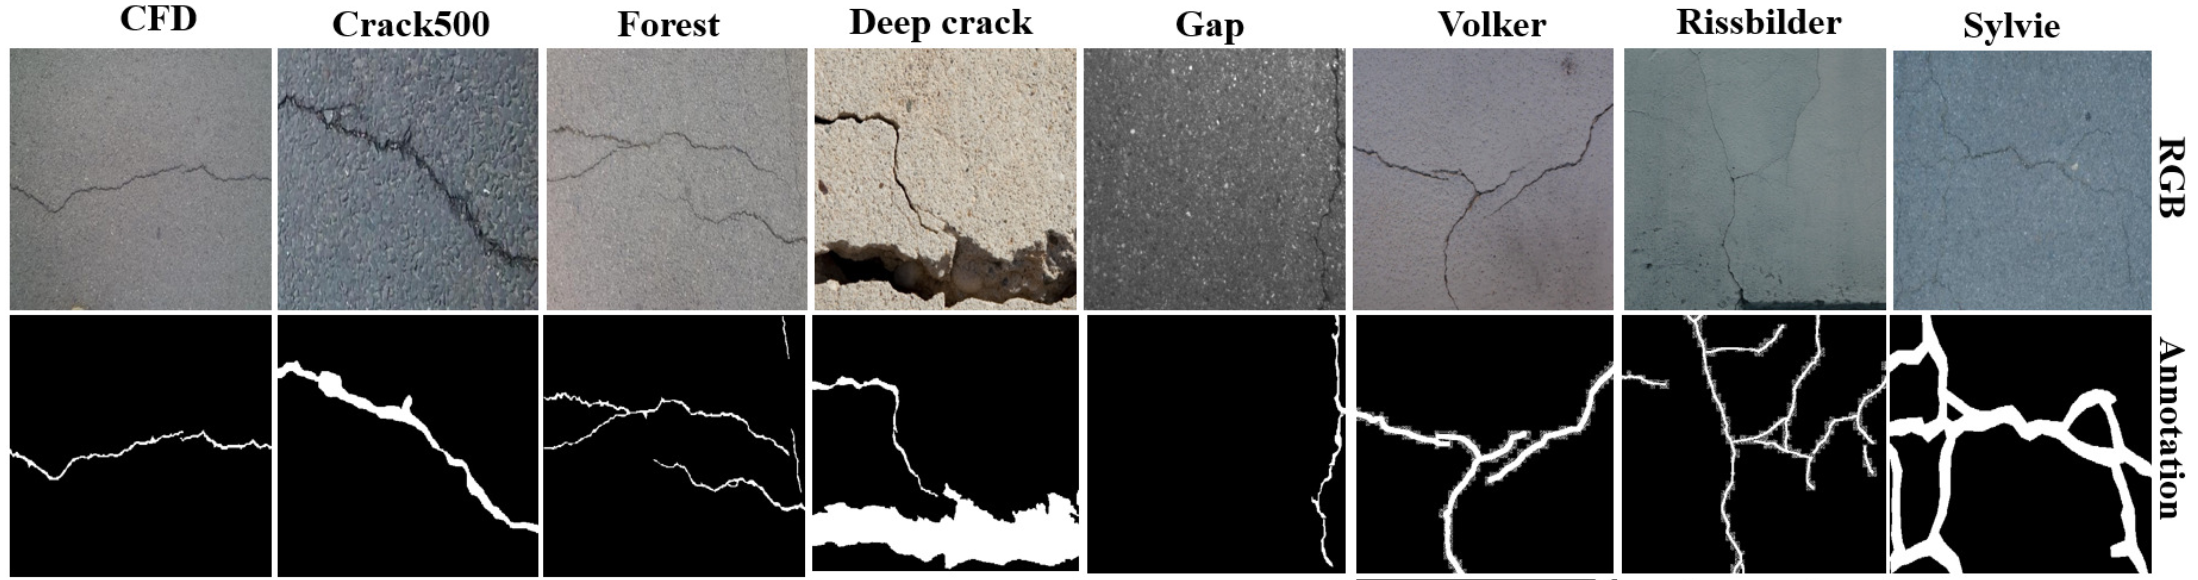
\includegraphics[width=1.05\linewidth]{res/crack-dataset.png}
    \caption{Crack dataset samples}
    \label{fig:crack-dataset}
\end{figure}
\end{frame}

\begin{frame}{Our Architecture}
    \vspace{0.1cm}
    \begin{figure}
        \centering
        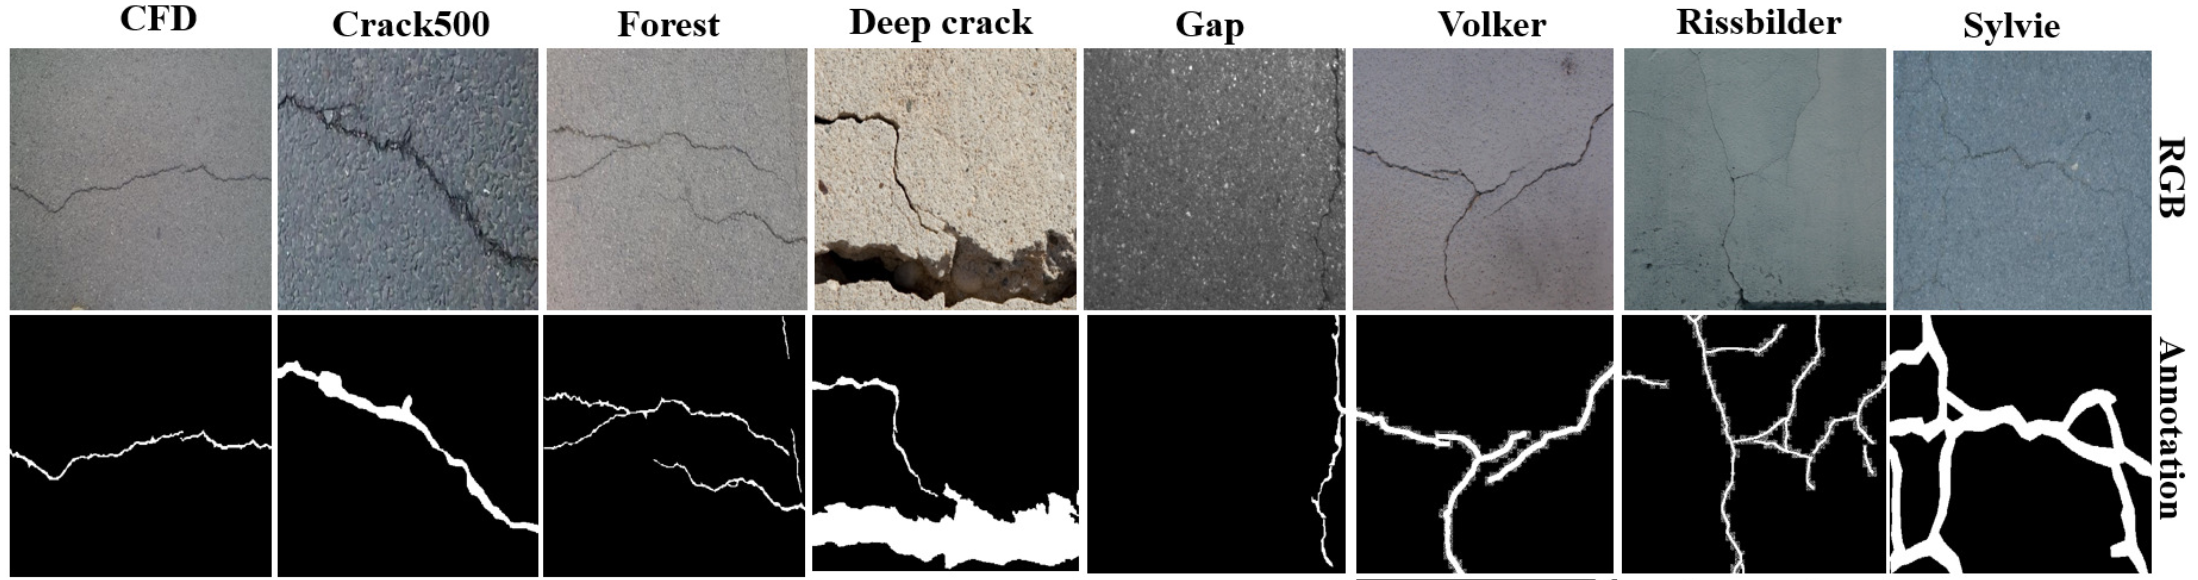
\includegraphics[width=1.05\linewidth]{res/crack-dataset.png}
        \caption{Crack dataset samples}
        \label{fig:crack-dataset}
    \end{figure}
    \end{frame}

\begin{frame}{SCMNet Architecture}
    \vspace{0.1cm}
    \begin{figure}
        \centering
        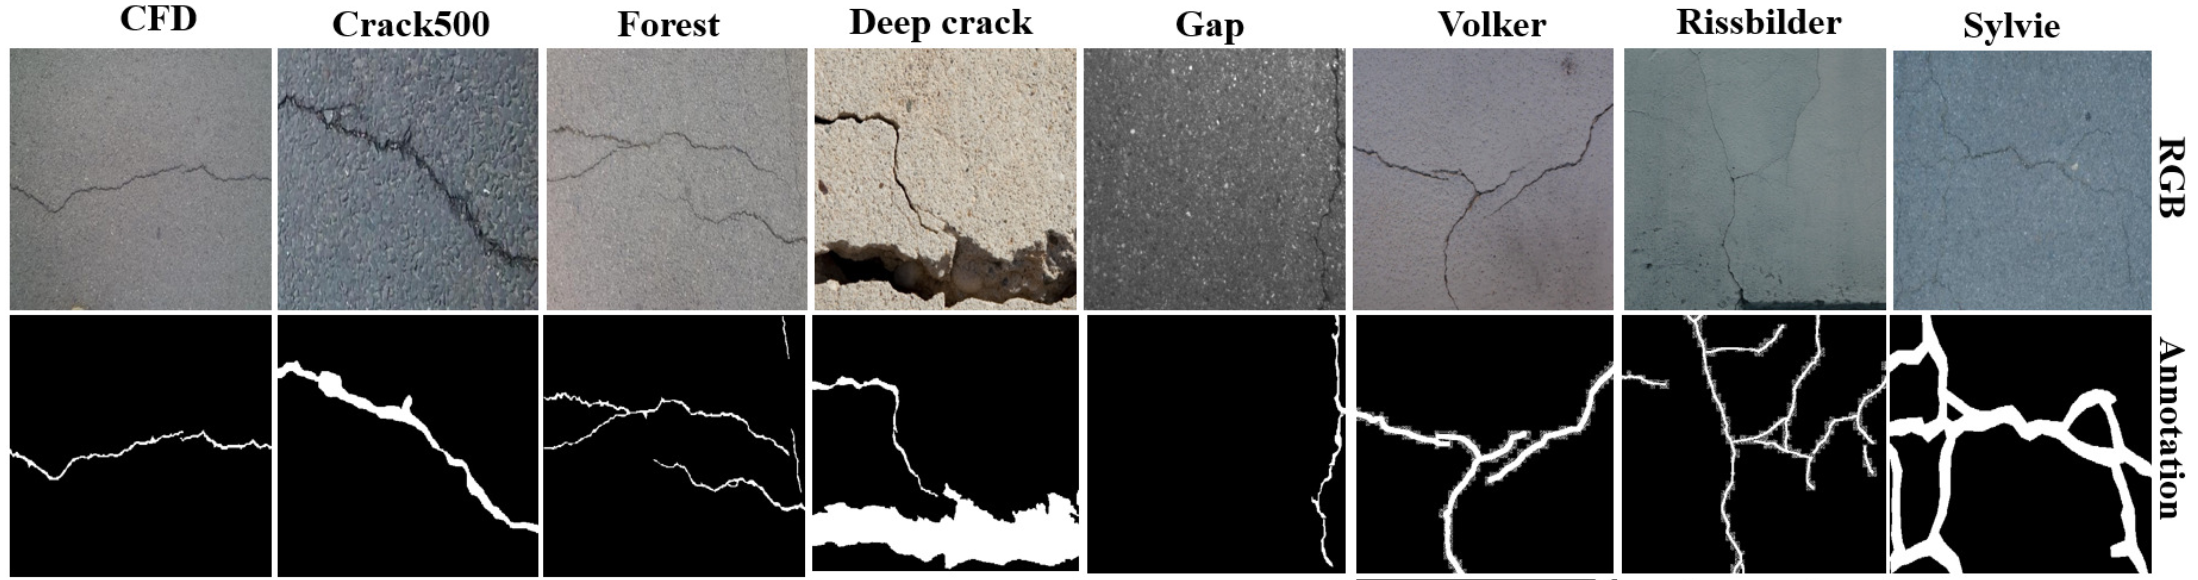
\includegraphics[width=1.05\linewidth]{res/crack-dataset.png}
        \caption{Crack dataset samples}
        \label{fig:crack-dataset}
    \end{figure}
    \end{frame}

% ---------------------------------------------------------------------------
%% ---------------------------------------------------------------------

%% ---------------------------------------------------------------------------
% Reference frames
% \begin{frame}[t,allowframebreaks]
%     \frametitle{References}
%     \printbibliography
% \end{frame}

%% ---------------------------------------------------------------------------
% Final frame
\begin{frame}{}
    \centering
    \huge{\textbf{\example{Thank you!}}}
    
    \vspace{1cm}
    
    \Large{\textbf{Contact:}}
    \newline
    \vspace*{0.5cm}
    \large{\email{tanmay.singha@postgrad.curtin.edu.au}}
    \large{\email{moritz.bergemann@student.curtin.edu.au}}
\end{frame}

\end{document}